% =========================================================================
% Capítulo 2: Cinética de la partícula
% Tema 01: Dinámica de la partícula
% Problema 17: Partícula en hélice circular
% Origen: Ayudantía 1, 2026
% =========================================================================
\subsubsection{Partícula en hélice circular}

Una partícula de masa $m$ se mueve a lo largo de una hélice circular de radio $R$ y ángulo de inclinación constante $\phi$, como se muestra en la \textbf{Figura \ref{fig:helice_particula}}. La ecuación de la hélice en coordenadas cilíndricas se define como:
\begin{equation}
    z = R \theta \tan \phi
\end{equation}
Sabiendo que la gravedad actúa en dirección vertical hacia abajo, y que las condiciones iniciales son $\theta(t=0)=\theta_0$ y $\dot{\theta}(t=0)=\dot{\theta}_0$, realice lo siguiente:

\begin{enumerate}
    \item Defina los marcos de referencia y sistemas de coordenadas adecuados.
    \item Determine y analice la cinemática de la partícula, expresando su velocidad y aceleración en términos de $\theta$.
    \item Determine y analice la cinética de la partícula para obtener la ecuación diferencial de movimiento en términos de $\theta$ utilizando el teorema de Trabajo y Energía.
    \item Determine el desplazamiento de la partícula cuando alcanza la máxima altura en la hélice.
\end{enumerate}

\begin{figure}[!ht]
    \centering
    \begin{tikzpicture}[>=Latex, scale=1.5]
        % --- Parámetros ---
        \def\R{1.2}      % Radio del cilindro
        \def\H{2.3}      % Altura del cilindro
        \def\phiang{15}  % Ángulo de inclinación

        % --- 1. Dibujo del Cilindro ---
        % Elipse inferior (fondo)
        \draw[dashed, gray] (\R, 0) arc (0:180:{\R} and 0.4);
        % Elipse superior
        \draw[thick, fill=gray!10] (0, \H) ellipse ({\R} and 0.4);
        % Paredes laterales
        \draw[thick] (-\R, 0) -- (-\R, \H);
        \draw[thick] (\R, 0) -- (\R, \H);
        % Elipse inferior (frente)
        \draw[thick] (-\R, 0) arc (180:360:{\R} and 0.4);

        % --- 2. Hélice ---
        \draw[thick, domain=0:7*pi, samples=100, smooth] 
            plot ({\R*cos(\x r)}, {0.1*\x + 0.15*\R*sin(\x r)});
        
        % --- 3. Partícula y Vectores ---
        % Posición de la partícula P (en un punto de la curva)
        \coordinate (P) at ({\R*cos(2.3*pi r)}, {0.1*2.3*pi + 0.15*\R*sin(2.3*pi r)});
        \coordinate (PProy) at ({2*\R*cos(2.44*pi r)}, { 2*0.15*\R*sin(2.44*pi r)});
        \shadedraw[ball color=gray!30] (P) circle (4pt) node[] {$m$};
        
        % Referencias de radio y ángulos en la base
        \coordinate (O) at (0,0);
        \draw[dashed] (O) -- (\R, 0) node[midway, below] {$R$};
        \draw[thick, ->] (O) -- (PProy);
        \draw[->] (0.4, 0) arc (30:60:0.5) node[midway, right] {$\theta$};
        \filldraw (O) circle (1pt) node[below] {$O$};

        % --- 4. Ángulo de inclinación phi ---
        \begin{scope}[shift={(0.25, 1.52)}, blue!30!black] 
            \draw[dashed] (0, 0) -- (0.9, 0);          % Horizontal
            \draw[thick] (0, 0) -- (\phiang:0.9);      % Pendiente (usando coordenadas polares)
            \draw[-] (0.4, 0) arc (0:\phiang:0.4);    % Arco del ángulo
            \node at (0.5*\phiang:0.8) {$\phi$};       % Etiqueta
        \end{scope}

        % --- 5. Gravedad ---
        \draw[->, thick] (2.0, 2.5) -- (2.0, 1.8) node[midway, right] {$\mathbf{g}$};

    \end{tikzpicture}
    \caption{Esquema de una partícula de masa $m$ recorriendo una trayectoria helicoidal sobre un cilindro de radio $R$.}
    \label{fig:helice_particula}
\end{figure}

% --- SOLUCIÓN ---------------------------------------------------------------
\begin{solucion}{Partícula en hélice circular}

\textbf{Marcos de referencia y Sistemas de Coordenadas}\\
Lo primero, como en todo ejercicio, es definir los marcos de referencia.
\begin{itemize}
    \item $\mathcal{N}$: el suelo $\longrightarrow\{\vec{e}_x;\vec{e}_y;\vec{e}_z\}$
    \item $\mathcal{A}$: centro $O$-proyección de $P$ $\longrightarrow\{\vec{e}_r;\vec{e}_\theta;\vec{e}_z\}$
\end{itemize}

\begin{center}
\begin{tikzpicture}[scale=0.8]
    \Polaresrtz{\theta}{e}{e}{azul}{myred}
    \node[above right] at (35:2) {$P$};
\end{tikzpicture}
\end{center}

\begin{equation*}
\begin{split}
    \vec{e}_r&=\cos\theta\,\vec{e}_x+\sin\theta\,\vec{e}_y\\
    \vec{e}_\theta&=-\sin\theta\,\vec{e}_x+\cos\theta\,\vec{e}_y\\
    \vec{e}_z&=\vec{e}_z
\end{split}
\end{equation*}

\subsubsection*{Cinemática de la partícula}
\textbf{Posición}\\
Como siempre, para obtener la velocidad de algún punto respecto a un marco inercial partimos por la posición; en este caso la de la partícula $P$ es
$$\vec{r}_P=R\vec{e}_r+z\vec{e}_z$$
Y necesitamos encontrar $z$ en términos de cosas conocidas. Para esto ocupamos el ángulo de inclinación $\phi$: si nos vamos al borde del cilindro tenemos un triángulo en el cual el cateto inferior corresponde a la cantidad de vueltas que ha dado la partícula (también se puede ver diferencialmente como un pequeño cambio; la distancia recorrida es $R\,d\theta$), que se puede representar como $R\theta$, donde recordemos que $\theta$ es el ángulo en radianes. Falta el otro cateto, que corresponde a cuánto ha subido la partícula ($z$) respecto a cuánto se ha recorrido ($R\theta$).
\begin{center}
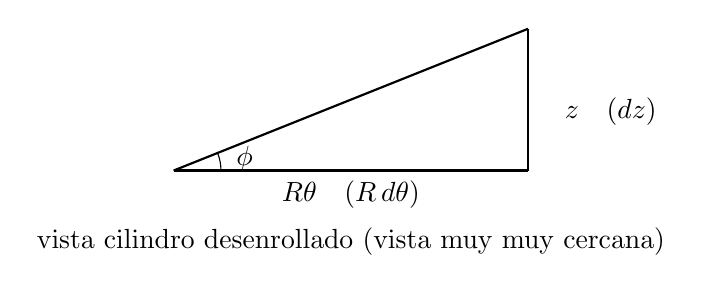
\begin{tikzpicture}[scale=1.5]
  \draw[thick] (0,0) -- (3,1.2); % hipotenusa
  \draw[thick] (0,0) -- (3,0);   % base
  \draw[thick] (3,0) -- (3,1.2); % lado
  \draw[dashed] (0,0) -- (0.8,0);
  \draw[dashed] (0,0) -- (0.8,0.32);
  \draw[-] (0.4,0) arc (0:21:0.4);
  \node at (0.6,0.1) {$\phi$};
  \node at (1.5,-0.6) {vista cilindro desenrollado (vista muy muy cercana)};
  \node at (3.7,0.5) {$z\quad(dz)$};
  \node at (1.5,-0.2) {$R\theta \quad(R\,d\theta)$};
\end{tikzpicture}
\end{center}
$$\tan\phi=\dfrac{z}{R\theta}=\dfrac{dz}{R\,d\theta}\quad\longrightarrow\quad z=R\theta\tan\phi$$

\textbf{Velocidad}\\
La velocidad es la derivada temporal de la posición desde un punto fijo.
% NOTA PARA REVISIÓN (agente B): el zip escribe der{(R e_r + R)}; por contexto debería ser R e_r + z e_z.
$$\marc{\vec{v}_P}{N}=\der{\vec{r}_{P}}{N}=\der{(R\vec{e}_r+R)}{N}{}= R\der{\vec{e}_r}{N}{}+R\dot\theta\tan\phi\,\vec{e}_z$$

\patotruco{No es necesario usar el teorema del transporte completo: usamos el trucazo (la demostración está en la Ayudantía 5). Como $\vec{e}_r$ y $\vec{e}_\theta$ giran solo en torno a $\vec{e}_z$, basta con $\dot{\vec{e}}_r=\dot\theta\vec{e}_\theta$ y $\dot{\vec{e}}_\theta=-\dot\theta\vec{e}_r$.}

Derivadas temporales de $\vec{e}_r$ y $\vec{e}_\theta$:
$$\transport{\vec{e}_r}{N}{A}=\dot\theta\vec{e}_z\times\vec{e}_r=\dot\theta\vec{e}_\theta$$
$$\transport{\vec{e}_\theta}{N}{A}=\dot\theta\vec{e}_z\times\vec{e}_\theta=-\dot\theta\vec{e}_r$$
y finalmente
$$\marc{\vec{v}_P}{N}=R\dot\theta\,\vec{e}_\theta+R\dot\theta\tan\phi\,\vec{e}_z$$

\textbf{Aceleración}\\
Al igual que antes, podemos simplemente derivar la velocidad:
$$\marc{\vec{a}_P}{N}=\der{\marc{\vec{v}_P}{N}{}}{N}{}=\der{\left(R\dot\theta\vec{e}_\theta+R\dot\theta\tan\phi\,\vec{e}_z\right)}{N}{}=(-R\dot\theta^2)\vec{e}_r+ R\ddot\theta\,\vec{e}_{\theta}+R\ddot\theta\tan\phi\,\vec{e}_z$$

\subsubsection*{Cinética}
\textbf{Diagrama de cuerpo libre}\\
Siempre se parte por un DCL, analizando las fuerzas que afectan a la masa. Recuerden que cada vez que eliminamos algo del DCL lo tenemos que reemplazar por una fuerza.
\begin{center}
\begin{tikzpicture}[>=Latex, scale=1.2]
    \shadedraw[ball color=gray!30] (0,0) circle (0.3) node {$m$};
    \draw[->, thick, azul] (0,0.3) -- (0,1.2) node[above] {$N_n$};
    \draw[->, thick, azul] (0.25,0.17) -- (1.2,0.75) node[above right] {$N_b$};
    \draw[->, thick, myred] (0,-0.3) -- (0,-1.2) node[below] {$mg$};
\end{tikzpicture}
\end{center}
Después del DCL se caracteriza cada fuerza vectorialmente:
$$\vec{F}_g=-mg\,\vec{e}_z$$
$$\vec{N}=N_b\vec{e}_b+N_n\vec{e}_n$$
En este caso no es necesario obtener las direcciones normal y binormal, porque más adelante se irán.

\textbf{Ecuación diferencial}\\
Ahora aplicamos el teorema de Trabajo y Energía. ¿Qué nos dice? (Discrepo con el nombre, porque en realidad es la derivada, pero cosas de la vida.) El teorema nos dice que la derivada (el cambio) de la energía cinética es igual a la potencia de las fuerzas.
$$\marc{P}{N}=\dfrac{d}{dt}(\marc{E_k}{N}{})$$
$$\marc{P}{N}=\marc{\vec{v}_P}{N}\cdot\sum \vec{F}$$
$$\marc{E_k}{N}=\dfrac{1}{2}m \marc{\vec{v}_P}{N}\cdot\marc{\vec{v}_P}{N}=\dfrac{1}{2}m \left(\marc{\vec{v}_P}{N}\right)^2$$
Reemplazando se tiene que
$$\marc{P}{N}=(-mg\vec{e}_z+N_b\vec{e}_b+N_n\vec{e}_n)\cdot\marc{\vec{v}_P}{N}\quad\longrightarrow\quad-mgR\dot\theta\tan\phi$$
% NOTA PARA REVISIÓN (agente B): en el zip la energía cinética se escribe con (R theta')tan^2(phi) en lugar de
% (R theta' tan(phi))^2; debería ser T = (1/2) m R^2 theta'^2 (1+tan^2 phi). Se deja tal cual.
$$\dfrac{d}{dt}(\marc{E_k}{N}{})=\dfrac{d}{dt}\left(\dfrac{1}{2}m((R\dot\theta)^2+(R\dot\theta)\tan^2\phi)\right)=mR\dot\theta (R\ddot\theta)(1+\tan^2\phi)$$
En la parte de las normales, se van; esto se puede ver claramente cuando expreso la velocidad como $\marc{v_P}{N}\vec{e}_t$ y hago el producto punto con la normal: da 0. Siguiendo con la igualdad se tiene que
$$mR\dot\theta (R\ddot\theta)(1+\tan^2\phi)=-mgR\dot\theta\tan\phi$$
$$m(R\ddot\theta)(1+\tan^2\phi)=-mg\tan\phi$$
\respuesta{$\displaystyle \ddot\theta=-\dfrac{g\tan\phi}{R(1+\tan^2\phi)}$}

\subsubsection*{Desplazamiento a máxima altura}
Se busca la máxima altura; para encontrarla tenemos que ver para qué valor de $\theta$ se consigue el máximo de $z=R\theta\tan\phi$. Podemos derivar e igualar a 0; de ahí se obtiene que en el punto de máxima altura $\dot\theta=0$. Con esta información podemos integrar el teorema de trabajo y energía (que ahora sí tiene sentido con el nombre; por eso, según yo, es el teorema integrado el que debería tener ese nombre).
$$\int_{0}^{t_f}\marc{P}{N}dt=\int_0^{t_f}\dfrac{d\left(E_k\right)}{dt}dt$$
$$\int_{0}^{t_f}-mgR\dot\theta\tan\phi\,dt=E_f-E_i$$
A mano izquierda hacemos un cambio de variable $\theta=f(t)$, mientras que al lado derecho tenemos la energía cinética final e inicial. Del análisis anterior sabemos que $\dot\theta=0$ en el punto que nos interesa (mayor altura), así que la energía cinética final es 0, y la inicial es, para $t=0$,
% NOTA PARA REVISIÓN (agente B): en el zip falta el factor 1/2 en E_i (debería ser (1/2) m R^2 theta'_0^2 (1+tan^2 phi)),
% lo que duplica theta_f - theta_0 y la componente z del desplazamiento. Se deja tal cual.
$$E_i=mR^2\dot\theta_0^2(1+\tan^2\phi)$$
$$\int_{0}^{t_f}-mgR\dot\theta\tan\phi\,dt\quad\dot\theta=\dfrac{d\theta}{dt}\quad\longrightarrow\quad\int_{\theta_0}^{\theta_f}-mgR\tan\phi\,d\theta=-mgR\tan\phi\,(\theta_f-\theta_0)$$
$$-mR^2\dot\theta_0^2(1+\tan^2\phi)=-mgR\tan\phi\,(\theta_f-\theta_0)$$
$$\theta_f = \theta_0 +\frac{R\,\dot{\theta}_0^2\,\bigl(1 + \tan^2\phi\bigr)}{g\,\tan\phi}$$
Con esto basta con evaluarlo en el desplazamiento de una partícula, que se define de manera más profesional como
$$\int_{t_i}^{t_f}\marc{\vec{v}}{N}dt$$
pero como la velocidad es la derivada de la posición, basta con evaluar en los extremos de la función posición:
\respuesta{$\displaystyle \vec{r}_{t_f}-\vec{r}_{t_i}=R\left(\cos\theta_f-\cos\theta_0\right)\vec{e}_x+R\left(\sin\theta_f-\sin\theta_0\right)\vec{e}_y+\frac{R^2\,\dot{\theta}_0^2\,\bigl(1 + \tan^2\phi\bigr)}{g}\vec{e}_z$}

\end{solucion}
